\chapter{Grundlagen von CYBOP}

  \section{�berblick}

    CYBOP steht f�r \emph{Cybernetics Oriented Programming}. Laut \cite{defkybernetik}
    ist Kybernetik folgenderma�en definiert:
    \begin{quote}
      Forschungsrichtung, die vergleichende Betrachtungen �ber
      Gesetzm��igkeiten im Ablauf von Steuerungs- und Regelungsvorg�ngen in Technik, 
      Biologie und Soziologie anstellt. 
    \end{quote}
    Kybernetik ist also eine Richtung die versucht das Verhalten und die Abstraktion 
    von einzelnen Systemen zu betrachten und zu vergleichen. Die Programmierung  
    von Anwendungssystemen wird von Menschen realisiert. Darum ist es nahe liegend, die 
    Programmierung (Beschreibungssprache) dem menschlichen Denken entsprechend zu modellieren. 
    
    Laut \cite{chepaper} gibt es folgende Prinzipien f�r das menschliche Denken:
    \begin{quote}
      Fundamental principles of human thinking are Discrimination,
      Categorization and Composition. The abstractions
      they deliver are Item, Category and Compound.
    \end{quote}
    
    CYBOP versucht nicht menschliches Denken nachzubilden, wie es der Begriff suggerieren k�nnte 
    oder wie der Begriff auch in dem Bereich K�nstliche Intelligenz verwendet wird, sondern 
    die Beschreibungssprache soll dem menschlichen Denken entsprechen. 

   \section{Discrimation/Items}
   
     Der Mensch versucht seine Umwelt zu verstehen. Zur Unterscheidung seiner Umwelt 
     gibt es in der Psychologie den Begriff \emph{Discrimination}.
     Dabei zergliedert der Mensch seine Umwelt in kleine Teile. Die Abbildungen 
     der realen Umwelt auf diese kleinen Teile werden in CYBOP \emph{Items} genannt. 
     Die \emph{Items} sind kontextabh�ngig. F�r verschiedene Aufgaben werden auch unterschiedliche 
     \emph{Items} gebildet, je nachdem welche Parameter f�r die Aufgaben relevant sind. 
     
     Der Mensch kann nur mit solchen Abbildungen umgehen, da er nie die
     Umwelt in ihrer Komplexit�t verstehen kann und dies f�r die L�sung  
     von Aufgaben auch nicht braucht. 
     Das menschliche Denken kann nur mit Modellen der Umwelt umgehen, 
     aber nie mit der gesamten realen Umwelt. 
  
  \section{Categorization/Category}
  
    Unter \emph{Categorization} versteht wir in diesem Zusammenhang die F�higkeit des Menschen
    verschiedene Teile auf Grund bestimmter Merkmale zu Gruppen zusammenzufassen. 
    In CYBOP wird dies \emph{Category} genannt. 
    In der \emph{Category} wird eine "`is-a-Beziehung"' beschrieben. Dies bedeutet, ein Teil geh�rt
    auf Grund spezieller Eigenschaften zu einer bestimmten Gruppe. 
    Die Gruppierungen k�nnen unterschiedlicher Natur sein. Ein einfaches Beispiel w�re 
    die Kategorie Mensch. Zu dieser Kategorie w�rden z.B. Afrikaner, Europ�er usw. 
    z�hlen.     
    
  \section{Composition/Compound}
  
    Teile k�nnen zu gr��eren Teilen zusammengefasst werden. Dieses Prinzip nennt man 
    \emph{Composition} und verk�rpert eine "`has-a-Beziehung"'. Die kleinsten 
    nicht teilbaren Teile nennt man Items. Wir wissen aber,
    das Teilen in der Regel weiter zerlegt werden k�nnen. Darum verstehen wir hier unter kleinsten nicht 
    teilbaren Teilen eine f�r die Aufgabe ausreichende Zerlegung. Die Abstraktion in CYBOP
    von einer \emph{Composition} ist das \emph{Compound}.
    Letzten Endes kann man also sagen, die Composition (lat. compositio = Zusammengesetztes) 
    ist ein Zusammenf�gen 
    von \emph{Items} oder anderen \emph{Compounds} zu etwas Gr��erem. 
    
  \section{Zusammenhang der Prinzipien}
  
    In der Abbildung \ref{human_thinking_figure} wird der Zusammenhang zwischen den gerade 
    beschriebenen Prinzipien von \emph{Human Thinking} verdeutlicht.
    Dies ist von \cite{chepaper} entnommen.
    \begin{figure}[H]
      \begin{center}
        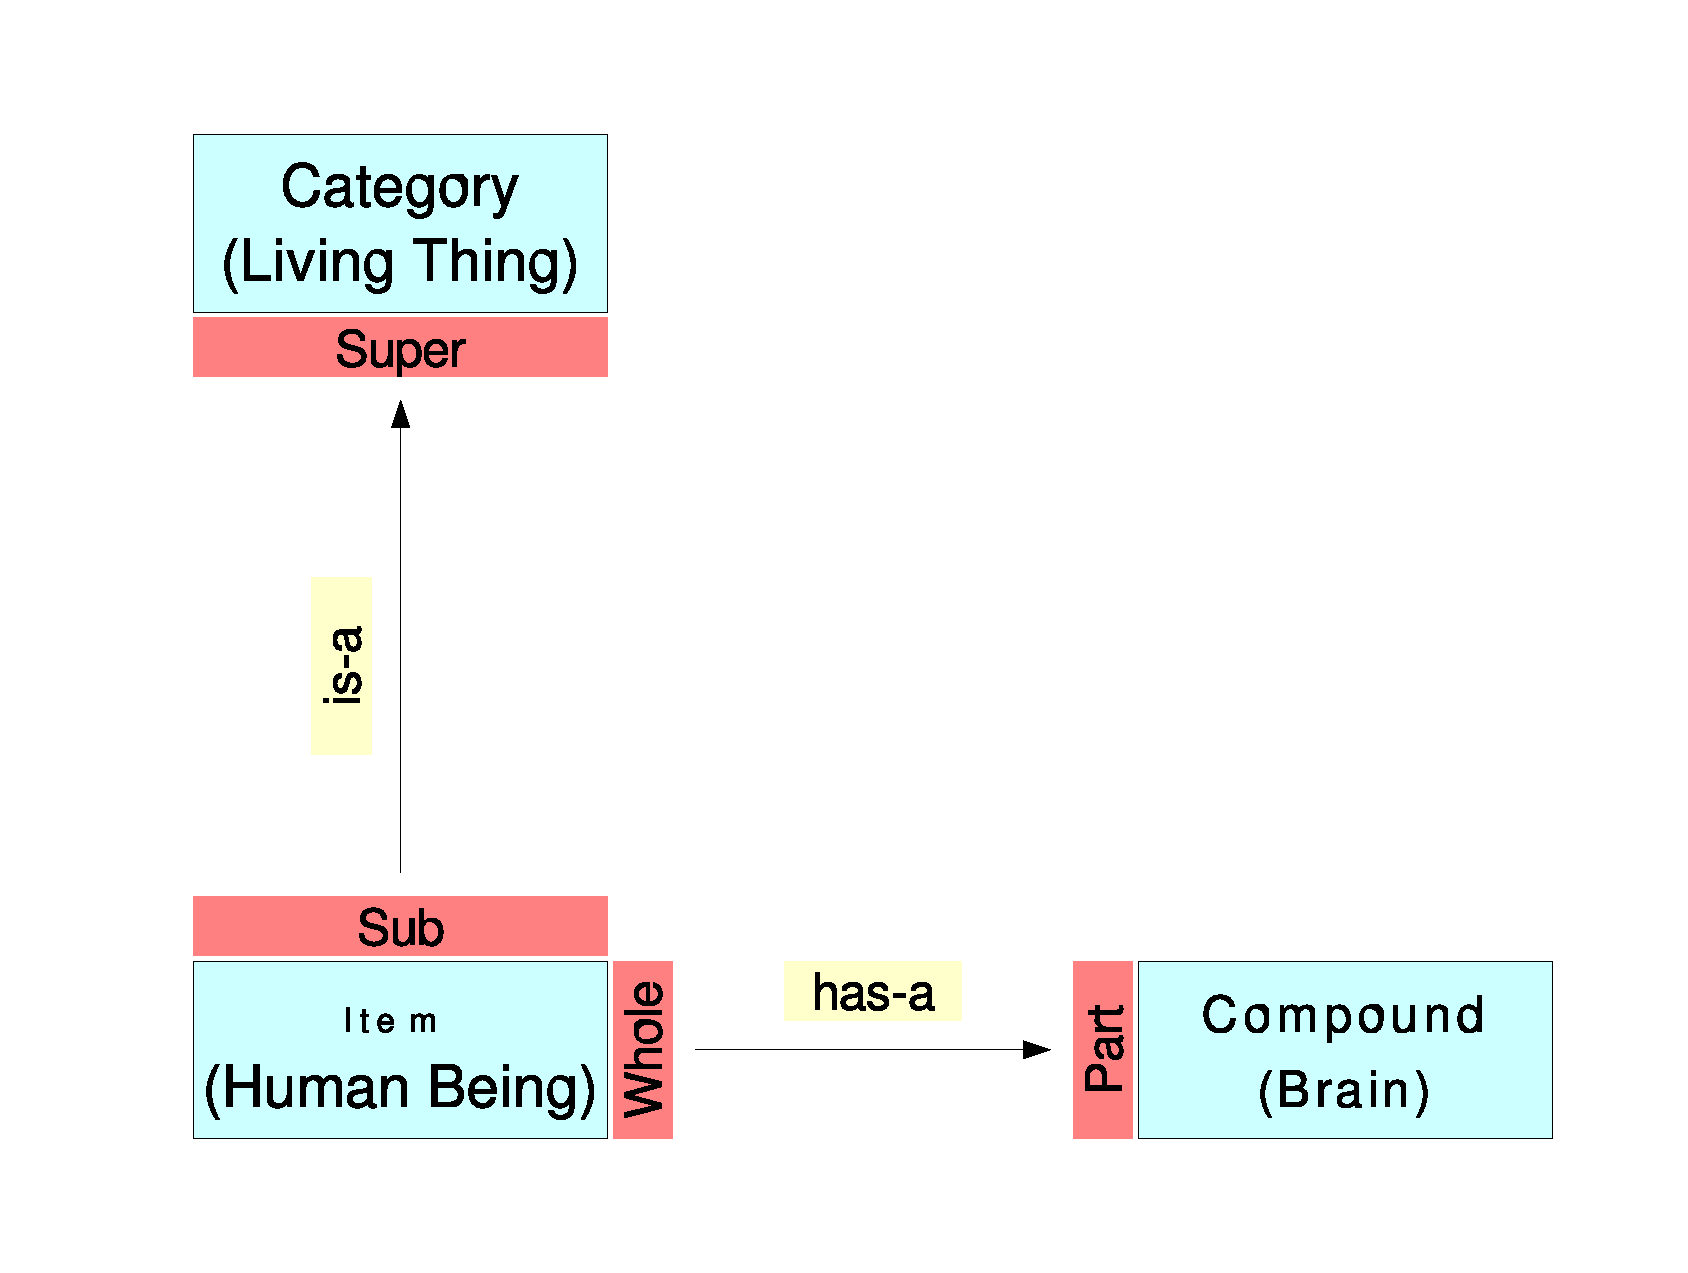
\includegraphics[width=10cm]{images/human_thinking.eps}
        \caption{Human Thinking}
        \label{human_thinking_figure}
      \end{center}
    \end{figure}
    
    \emph{Items} k�nnen �ber die "`has-a-Beziehung"' ein \emph{Compound} bilden und werden �ber die 
    "`is-a-Beziehung"' zu einer \emph{Category} zusammen gefasst. Wie sind diese Prinzipien in CYBOL umgesetzt?
    Jedes Template bzw. Laufzeitmodell vom Template repr�sentiert ein diskretes \emph{Item} bzw. 
    ein diskretes \emph{Compound}, was wiederum aus disketen \emph{Items} oder 
    \emph{Compounds} besteht. Die Abstraktion \emph{Category} ist in CYBOL nicht direkt als
    Beschreibung abgebildet, sondern muss
    �ber Operationen in CYBOL realisiert werden.
    
  \section{Architektur von CYBOP}
  
    CYBOP setzt sich aus verschieden Teilen zusammen. Dies beinhaltet einmal die Beschreibungssprache,
    dann einen Interpreter, der diese  Beschreibungssprache versteht und auf unterster Ebene 
    die Hardware, auf der die Operationen ausgef�hrt werden.
    
    \begin{itemize}
      \item Beschreibungssprache CYBOL \\
            Hier werden die Modelle beschrieben. Dazu geh�ren das Domain-Wissen, die Anwendungslogik
            und die Beschreibung der Oberfl�che f�r verschieden Ausgabemedien.
      \item Interpreter CYBOI \\
            Dies ist das Herzst�ck von CYBOP. Hier wird die Sprache CYBOL interpretiert. Dazu werden die Modelle
            gelesen, verarbeitet und f�r die verschiedenen Ausgabemedien die Anwendung generiert.
      \item Hardware \\
            Damit eine Anwendung funktioniert muss sie mit der Hardware zusammen arbeiten.  Dies muss durch den 
            CYBOP - Interpreter gew�hrleistet werden.
    \end{itemize}
    
    Die Beschreibungssprache CYBOL und der Interpreter CYBOI werden in den n�chsten Kapitel beschrieben. 
    Der Abschnitt Hardware ist f�r die Diplomarbeit nicht relevant.
    